\documentclass[conference]{IEEEtran}
\IEEEoverridecommandlockouts
% The preceding line is only needed to identify funding in the first footnote. If that is unneeded, please comment it out.
\usepackage{cite}
\usepackage{amsmath,amssymb,amsfonts}
\usepackage{algorithmic}
\usepackage{graphicx}
\usepackage{textcomp}
\usepackage{xcolor}
\usepackage{amsfonts,amsmath, amssymb}
%\usepackage[spanish]{babel}
\usepackage{fancyhdr}
%\usepackage[none]{hyphenat}
\usepackage[nottoc, notlot, notlof]{tocbibind}
\usepackage{cite}
\usepackage{physics}
\usepackage{bm}
\usepackage{enumitem}
\usepackage{a4wide}
\usepackage{dsfont}
\usepackage{ amssymb }
\usepackage{cite}
\usepackage[rightcaption]{sidecap}
\usepackage{graphicx}
\usepackage{algorithm}
\usepackage{algorithmic}
\usepackage{ragged2e}
\usepackage{pdfpages} 
\usepackage{csquotes}
\usepackage{listings}
\usepackage{hyperref}
\hypersetup{
    colorlinks=true,
    linkcolor=blue,
    filecolor=blue,      
    urlcolor=blue,
    citecolor=blue,
}
\def\BibTeX{{\rm B\kern-.05em{\sc i\kern-.025em b}\kern-.08em
    T\kern-.1667em\lower.7ex\hbox{E}\kern-.125emX}}
\begin{document}

\title{Correlation between atom and cavity emissions in a driven Jaynes-Cummings system\\
%{\footnotesize \textsuperscript{*}Note: Sub-titles are not captured in Xplore and
%should not be used}
\thanks{corresponding author e-mail: guillermopreisser@hotmail.com}
}

\author{\IEEEauthorblockN{Guillermo Preisser and Pablo Barberis Blostein}
\IEEEauthorblockA{\textit{Instituto de Investigaciones en Matemáticas Aplicadas y en Sistemas,
} \\
\textit{Universidad Nacional Autónoma de México, Ciudad Universitaria, 04510, CDMX, México.}\\
Dated: 15 August, 2019}
}

\maketitle

\begin{abstract}
We consider a driven Jaynes-Cummings system under weak coupling, which interacts with the environment through emissions from the atom and emissions that leak through one of the lateral cavity mirrors.  We fix the parameters of the model in order to stablish a dynamic in which the number of photons in the leaky cavity remain constant and, using quantum trajectory theory, we estimate the number of spontaneous emissions in the two-level atom – which will be measured from the upper side of the cavity – by measuring emissions that leak through one of the semi-transparent cavity mirrors. Studying the system further we find that the cavity generates a correlation between the emissions from the two sources.
\end{abstract}

%the recent advances?
\section{Introduction}
Spontaneous emission is a phenomenon that has been studied formally since early XX century \cite{10.2307/94746, 1917PhyZ...18..121E}. One of the main characteristics of spontaneous emission is that, while it is known that an atom will decay exponentially, the exact time of emission, as well as the direction in  which the photon is emitted, is random, which difficults its measurement. On the other hand, photons emitted from a stimulated cavity are easy to measure, partly due the fact that we know that they leave the cavity through one of the lateral mirrors \cite{326305, doi:10.1063/1.113345}. One of the main sources for single photons are two-level atoms. However, due to the randomness of the direction in which the photons are emitted, there are difficulties in managing such sources. To sort out this difficulty one could think of a physical arrangement, in which the two-level atom is coupled to the stimulated mode of a cavity, as it is shown in Fig. \ref{asa} (b). In this physical arrangement, which is known as the driven Jaynes-Cummings model, one could try to estimate the number of spontaneous emissions of the atom, which are emitted in the upper and lower directions of the system, by measuring the photons that leak through one of the cavity mirrors, on the lateral side. In the case that a correlation exists between the two quantities, this could turn useful in the manipulation of two-level atoms as single photon sources. 
\begin{center}
\begin{figure*}\label{asa}
\begin{center}
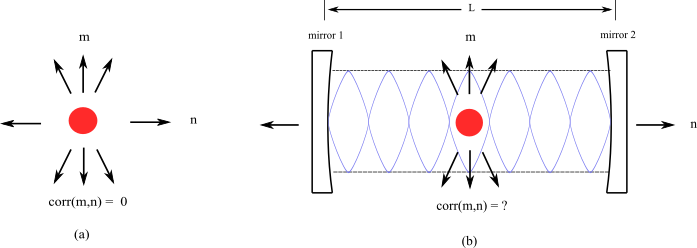
\includegraphics[scale = 0.65]{new_image_paper.png}
%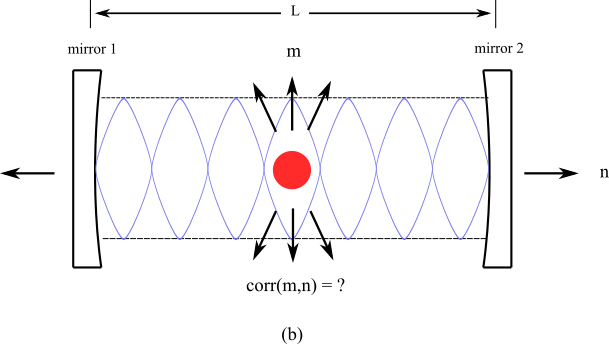
\includegraphics[scale = 0.45]{image_paper222.png}
\caption{\small{Physical arrangements of atom and atom in a cavity. In both of these arrangements we consider a source which stimulates the atom provoking it to spontaneously emit, once it decays. We consider a detector in two directions, and we keep a register of the number of photons measured in each direction. (a) In the case for the atom we don't expect a correlation between m (the number of photons measured in the upper side of the atom) and n (the number of photons measured in the right side of the atom); (b) for the atom in the cavity (a cavity with some loss rate) we study the possibility that the cavity generates a correlation between the emissions of the atom and the emissions of the cavity, which correspond to the emissions that leak through mirror 2.}} \label{probdisult}
\end{center}
\end{figure*}
\end{center}


It is easy to see why there would be no correlation between the directions of the emissions in the case for the two-level atom, without cavity. At the moment of modelling such physical system we consider a Markovian dynamic (i.e., the environment relaxes rapidly to an equilibrium state and on relevant timescales has no memory of previous interactions with the system \cite{daley2014quantum}). Given that the only way for a correlation to happen between the two emissions would be if one the emissions stay registered in the environment and, somehow, later influence the quantum system at a later time; by taking account of the Markovian dynamic we can have certainty that there is no direct correlation between the number of emissions of each source. Nevertheless, for the case of the atom coupled to a mode of a cavity, before a photon is emitted, it will most likely interact with the atom for some time. We consider the possibility that this interaction with the atom before the emission could contribute to the generation of a correlation between the emissions, which is what we study further in this paper.

In order to simulate quantum systems with dissipation and loss of coherence, like the one we deal with in this work, we use quantum trajectory theory. %Quantum trajectory was developed for various groups at the beginning of the 90's
One can define a quantum trajectory as the description of a continuously monitored quantum system conditioned on a particular past history of coherent evolution and collapse \cite{Carmichael1993Open}. These trajectories are simulated through a stochastic process, which define the times when the collapses occur.

In this work we estimate the number of spontaneous emissions by measuring stimulated emissions in an optical cavity and we calculate the existing correlation between the two emissions. This is done via quantum trajectories in which, by doing a large number of simulation and making a register of the number of spontaneous emissions and cavity emissions, we obtain probability distributions which relates these two quantities. We proceed in doing numerical calculations in order to prove that there is a correlation between two quantities, and we see how this correlation varies with respect to the cavity linewidth. \\


This article is set up as follows: A general overview of the driven Jaynes-Cummings model is presented in section two. In section three we obtain probability distributions that relate the number of spontaneous and cavity emissions. In section four we calculate the correlation between the two variables. Concluding remarks are given in section six.

%consideeron an initially ground state 0 photons

%\begin{center}
%\begin{figure}[t!]
%\begin{center}
%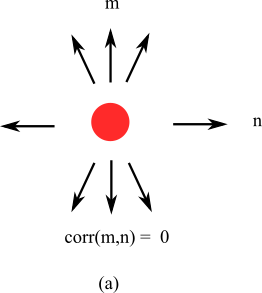
\includegraphics[scale = 0.45]{image_paper11.png}
%\caption{\small{Calculation of correlation using 500 time intervals, fixing $\expval{n} \approx 1$, $\gamma =$ 1.0, $g = $ 0.1, and with  $\mathcal{E} =  \kappa |\langle n \rangle|[1 + 2g^2/\gamma \kappa]$.}} \label{corrxy}
%\end{center}  
%\end{figure}
%\end{center}

%\begin{center}
%\begin{figure}[t!]
%\begin{center}
%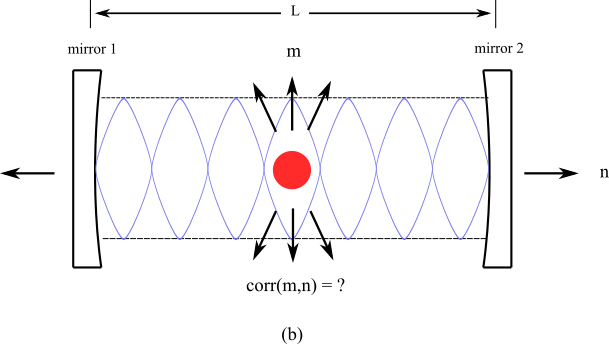
\includegraphics[scale = 0.45]{image_paper222.png}
%\caption{\small{Calculation of correlation using 500 time intervals, fixing $\expval{n} \approx 1$, $\gamma =$ 1.0, $g = $ 0.1, and with  $\mathcal{E} =  \kappa |\langle n \rangle|[1 + 2g^2/\gamma \kappa]$.}} \label{corrxy}
%\end{center}  
%\end{figure}
%\end{center}
\section{Driven Jaynes-Cummings model}
We consider a system consisting of a two-level atom, coupled to a mode of a cavity. The mode is driven by a coherent field resonant with the atom and the mode of the cavity. In order to account for dissipation one may use a non-hermitian Hamiltonian to describe the system \cite{bla}. Using this description for the system will turn useful at the moment of using quantum trajectory theory. Such Hamiltonian can be separated into hermitian and non-hermitian terms.
%\begin{equation}
%H = H_s - \frac{i\hbar}{2}\sum_m C^\dagger_n C_n .
%\end{equation}
The hermitian part of our Hamiltonian is given by $H_s$ which for the driven Jaynes-Cumming, under the rotating wave approximation, reads as
\begin{equation}
H_s = H_{at} + H_{cav} + H_{atcav} + H_{lascav}, \label{mainham}  
\end{equation}
where the atom and cavity terms are, respectively
\begin{subequations}
\begin{equation}
H_{at} = \tfrac{1}{2}\hbar \omega \sigma_z,    
\end{equation}
\begin{equation}
H_{cav} = \hbar \omega  a^\dagger a,  
\end{equation}
while the coupling between atom and cavity, and cavity and coherent field are
\begin{equation}
H_{atcav} = i\hbar g(a\sigma_+ - a^\dagger \sigma_-),    
\end{equation}
\begin{equation}
H_{lascav} = i\hbar \mathcal{E}(ae^{i\omega t} - a^\dagger e^{-i\omega t}),    
\end{equation}
\end{subequations}
where we introduced the coupling constant
\begin{equation}
g = \sqrt{\frac{\omega d^2}{2\hbar \epsilon_0 V_Q}},
\end{equation}
with the mode volume $V_Q$, dipolar coupling constant $d$, and $\epsilon_0$ is the permitivity of free space. $\mathcal{E}$ is a term proportional to the coherent field amplitude.
As for the non-hermitian part of our Hamiltonian, we have
\begin{equation} \label{nh}
H_{nh} = H_{dec} + H_{leak},
\end{equation}
where the terms corresponding to the spontaneous emission of the atom and the cavitty losses are
\begin{subequations}
\begin{equation}
H_{dec} = - i\hbar\frac{\gamma}{2}\sigma_+\sigma_-,
\end{equation}
\begin{equation}
H_{leak} = - i\hbar\kappa a^\dagger a.
\end{equation}
\end{subequations}
The annihilation operator $a$ of a single photon in the cavity, and the creation operator $a^\dagger$ obey $[a, a^\dagger] = 1$. The operators $\sigma_-, \sigma_+$  account for the atomic lowering and raising operators, respectively, and the operator $\sigma_z$ accounts for the population difference between the atomic levels. These operators obey $[\sigma_+, \sigma_-] = \sigma_z, \ [\sigma_\pm, \sigma_z] = \mp 2\sigma_\pm$. $\kappa$ and $\gamma$ are the cavity loss and spontaneous decay rate.\\ %With the Hamiltonian Eq. \eqref{mainham} we can write down the master equation for the driven Jaynes-Cummings model in its Lindblad form
%\begin{equation}
%\frac{\partial \rho}{\partial t} = -\frac{i}{\hbar} [H(t), \rho]  + \mathcal{L}_\kappa \rho + \mathcal{L}_{\gamma} \rho,
%\end{equation}
%where 
%\begin{equation}
%\mathcal{L}_\kappa  \rho =  \mathcal{D}[\sqrt{2\kappa}a] \rho, 
%\end{equation}
%and
%\begin{equation}
%\mathcal{L}_\gamma \rho = \ \mathcal{D}[\sqrt{\gamma}\sigma_-] \rho,
%\end{equation}
%where $\mathcal{D}$ is a superoperator that will act on the density matrix as
%\begin{equation}
%\mathcal{D}[C] = \frac{1}{2}[2C\rho C^\dagger - C^\dagger C \rho - \rho C^\dagger   C],
%\end{equation}
%where we identify $C$ as the jump operators which will be the ones that will cause the dissipation in the system when we work using quantum trajectory theory.
%\begin{figure*}[t!]
%\includegraphics[scale = 0.8]{phases.png}
%\end{figure*}
%\begin{SCfigure*}[0.9][!h] \label{figsis}

%\includegraphics[scale = 0.8]{phases2.png}
%\caption{\small{Trayectorias cuánticas de prueba correspondientes a la ecuación maestra \eqref{masterbioptical} en el límite de acoplamiento fuerte mostrando el número promedio de fotones: $g/\kappa = 10, \gamma/2\kappa =  1$, y (a) $  \mathcal{E}/\kappa = $ 3.0; (b) $\mathcal{E}/\kappa = $ 5.0; (c) $\mathcal{E}/\kappa = $ 9.0.}}
%\label{figsis}
%\end{SCfigure*}

\section{Estimation of spontaneous emissions}
In this section we obtain estimations for the number of spontaneous emissions by measuring stimulated emission in a cavity mode in the driven Jaynes-Cummings model, using quantum trajectory theory.
\subsection{Probability distributions of emissions}
In order to get the desired estimations, first we must obtain probability distributions that relate the number of spontaneous emissions of the atom with the emissions measured from the cavity. We achieve this by making a large number of quantum  trajectories from which we keep a record of the number of spontaneous emissions and cavity losses, relating the number of spontaneous emissions for each number of cavity loss and making a probability distribution out of the emission's register of the trajectories. 

In order to achieve this, following the procedure from quantum trajectory theory as it is explained in \cite{bla}. Starting with a state which represents a ground state of the atom with no photons in the cavity, $\ket{\phi(t = 0)} = \ket{\downarrow} \times \ket{0}$, we evolve it with the Schrödinger equation through some time $\delta t$, using a non-hermitian Hamiltonian of the form
\begin{equation}
H = H_s - \frac{i\hbar}{2}\sum_n C^\dagger_n C_n,
\end{equation}
where the operators $C_n$ are known as collapse operators.
Using a non-hermitian Hamiltonian will have as a consequence that the probability won't be conserved \cite{Sakurai:1167961}. The evolution of the state through the schrödinger equation will be interrupted by a quantum jump – an abrupt change on our state in which a photoemission has ocurred. The probability for such quantum jump to happen will be given by the collapse probability
\begin{equation} \label{probcol}
\delta p = \sum_n \delta p_n,
\end{equation}
where 
\begin{equation} \label{relprob}
\delta p_n = \delta t \bra{\phi (t)} C^\dagger_n C_n \ket{\psi (t)}.
\end{equation}
We use these collapse probabilities to simulate the quantum trajectories, where we compare the collapse probability of eq. \eqref{probcol} with a random number $\epsilon$, uniformly distributed between zero and one. In the case the condition $\delta p > \epsilon$ is fulfilled we simulate that a quantum jump has happened, by acting with one of the collapse operators. The operator with which we'll act on the state will be given according to the relative probabilities of eq. \eqref{relprob}. From the non-hermitian Hamiltonian of our system \eqref{nh} we are able to identify the corresponding collapse operators which are
\begin{figure}[!t] 
\centering
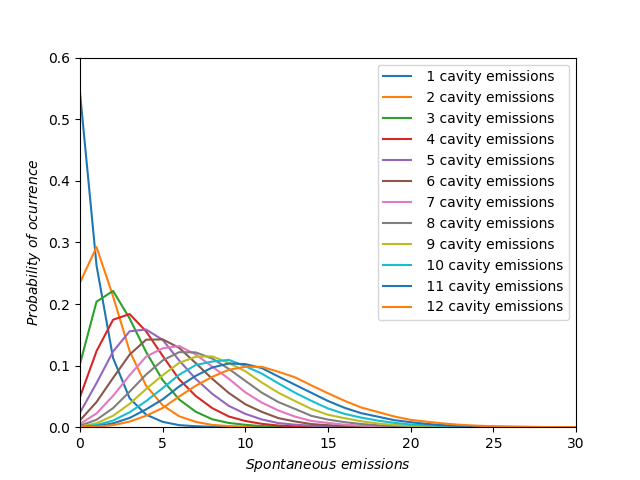
\includegraphics[scale = 0.5]{distributioneng.png}
\caption{\small{Probability distribution of spontaneous emissions for different number of cavity losses in a driven Jaynes-cummings model, doing $100,000$ quantum trajectory simulations, with parameters $\mathcal{E}  = \kappa = \gamma = g = 1$.}} \label{probdiss}
\end{figure}
\begin{subequations}
\begin{equation}
C_1 = \sqrt{\gamma}\sigma_-,
\end{equation}
\begin{equation}
C_2 = \sqrt{2\kappa}a.
\end{equation}
\end{subequations}
Using equation \eqref{probcol} one can easily identify the corresponding collapse probabilities of the system. Having identified the collapse operators and the collapse probability, we simulate quantum trajectories, in which we keep count of the number of quantum jumps for each collapse operator, relating the number of quantum jumps associated to spontaneous emissions for each number of quantum jumps associated to cavity emissions until we reach a maximum number of cavity emissions, which we establish. The procedure of register of emissions is summarized in algorithm \ref{alg1}. 

Realizing a large number of these trajectories, storing the registers in a matrix, where we keep track of the number of times that there were certain number of spontaneous emissions for each different number of cavity emission, enable us to obtain probability distributions that relate these two quantities.  

In Fig.\ref{probdiss} we see the probability of obtaining different number of spontaneous emissions for different number of cavity emissions. It is clear from the plot that our probability distributions are going to be more spread out as more time (and hence more cavity emissions) pass.


\begin{algorithm}[!t]
\caption{Pseudocode for register of cavity losses and atom's spontaneous emissions}
\label{alg1}
\begin{algorithmic}
\STATE $N$: number of temporal intervals
\STATE $N_A $: number of spontaneous emissions
\STATE $N_C$: number of cavity emissions
\STATE $N_{max}$: maximum number of cavity emissions
\STATE $N_{CA}$: matrix relating the number of cavity emissions with the number of spontaneous emissions
%\STATE $K [\equiv] contador$

\STATE
\STATE Initial conditions:
\STATE $N_A = 0; N_C = 0;$
\STATE $N_{CA} = \text{zeros}(N_{max},2);  k = 0;$ 
%\STATE $\delta p > \epsilon$
%\STATE $\ket{\phi (t = 0)} = \ket{0}\otimes \ket{\downarrow}$ 
\STATE 
%\end{enumerate}
%\IF $p^T_c \geq \epsilon $
%\compute casa
%\FORALL {$i$ in $S_i$}
%\IF
%\IF {$\delta p > \epsilon$}

%\FOR{$i = 1$ to N} 
%\STATE $\ket{ \phi^1(t + \delta t)} = e^{-iH\delta t/\hbar}\ket{\phi (t)}$
%\STATE$ \delta p_1 = \delta t\bra{\phi(t)}C^\dagger_1 C_1\ket{\phi(t)}$
%\STATE $ \delta p_2 =  \delta t\bra{\phi(t)}C^\dagger_2 C_2\ket{\phi(t)}$
%\STATE $\delta p = \delta p_1 + \delta p_2$
\FOR{$i = 1$ to N} 
\STATE $\ket{ \phi^1(t + \delta t)} = e^{-iH\delta t/\hbar}\ket{\phi (t)}$
\STATE$ \delta p_1 = \delta t\bra{\phi(t)}C^\dagger_1 C_1\ket{\phi(t)}$
\STATE $ \delta p_2 =  \delta t\bra{\phi(t)}C^\dagger_2 C_2\ket{\phi(t)}$
\STATE $\delta p = \delta p_1 + \delta p_2$
\IF {$\delta p > \epsilon$}
\IF{$ \tfrac{\delta p_1}{\delta p} > \epsilon$}
\STATE $\ket{\phi (t + \delta t)} = \frac{C_1 \ket{ \ \phi(t)}}{\sqrt \frac{\delta p_1}{\delta t}}$
\STATE $N_A = N_A + 1$
\ELSE
\STATE $\ket{\phi (t + \delta t)} = \frac{C_2 \ket{ \ \phi(t)}}{\sqrt \frac{\delta p_2}{\delta t}}$
\STATE $N_C = N_C + 1$
\STATE $N_{CA}[k+1,1] = N_C$
\STATE  $N_{CA}[k+1,2] = N_A$
\STATE $k = k+1$
\IF{$N_C == N_{max}$}
\STATE \textbf{\textit{break}}
\ENDIF
%\STATE $x$ was less than the minimum threshold
\ENDIF
\ELSE
\STATE $\ket{ \phi(t + \delta t)} = \frac{\ket{\phi^1 (t+ \delta t)}}{\sqrt{1-\delta p}}$
\STATE $t \ += \delta t$
\ENDIF
\ENDFOR
\RETURN  $N_{CA}$
%\STATE $t \ += \delta t$
%\ENDFOR
%\ENDIF
%\ENDIF
%\ENDFOR
%\end{enumerate}
\end{algorithmic}
%\caption{Algoritmo para obtener distribución de probabilidad de número de emisiones espontáneas}
\end{algorithm}



\begin{center}
\begin{figure*}[!t]\label{error2}
\begin{center}
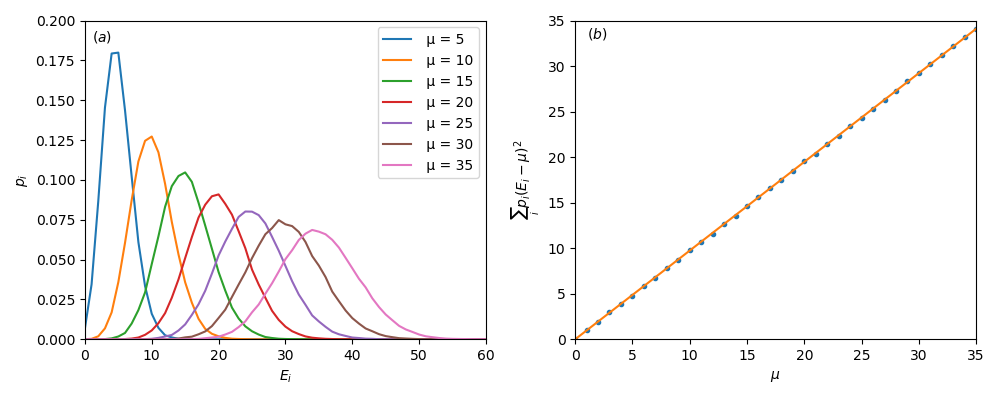
\includegraphics[scale = 0.55]{newerrorppp.png}
\caption{\small{(a) Probability distributions for different mean number of spontaneous emissions $\mu$; (b) Calculation of variance with respect to the mean number of sponatenous emissions $\mu$. In both cases we consider $\expval{n} \approx 1$, $\gamma = 1.0$ , $\kappa = g = 0.1$ and $\mathcal{E} =  \kappa |\langle n \rangle|[1 + 2g^2/\gamma \kappa]$.}} \label{probdisult}
\end{center}
\end{figure*}
\end{center}
\subsection{Extracting data from the probability distributions}
Due to the complex dynamic of the driven Jaynes-Cummings system \cite{Carmichael1993Open}, it is important to know the dynamic that the system undergoes at the moment of obtaining the probability distributions, in order to have a better physical understanding of our results. In this case we opt for fixing the number of photons in the cavity.


We do this by solving what is known as the Maxwell-Bloch equations, which give the dynamic of our system for the variables  $\expval{a}, \expval{\sigma_-}$ and $\expval{\sigma_z}$ that correspond to the cavity field, atomic coherence, and atomic inversion respectively \cite{Alsing_1991}. For the case of the driven Jaynes-Cummings system, these equations are given by
\begin{subequations} \label{maxbloch}
\begin{equation} \label{bloch1}
\dot{z} = (g/2)v + \mathcal{E} - \kappa z,
\end{equation}
\begin{equation} \label{bloch2}
\dot{v} = gmz - (\gamma/2)v,
\end{equation}
\begin{equation} \label{bloch3}
\dot{m} = -2g(z^*v + v^*z) - \gamma(m + 2),
\end{equation}
\end{subequations} 
where we defined  $z = e^{i\omega t}\expval{a}$, $v = 2e^{i\omega t}\expval{\sigma_-}$ and $m = 2\expval{\sigma_z}$. Solving for the case in which our variables are constant we can obtain steady state solutions \cite{gagniuc2017markov}.  From \eqref{bloch1} one can obtain the equation
\begin{equation} \label{chaf1}
\expval{a}_{ss} = \frac{\mathcal{E}e^{-i\omega t} + g\expval{\sigma_-}_{ss}}{\kappa}.
\end{equation}
While from \eqref{bloch2} and \eqref{bloch3} one obtains
\begin{equation} \label{chaf2}
\expval{\sigma_-}_{ss} = -\frac{2g}{\gamma}\frac{\expval{a}_{ss}}{1 + \frac{8g^2}{\gamma^2}|\expval{a}_{ss}|^2}.
\end{equation}
The requirement that both \eqref{chaf1} and \eqref{chaf2} are valid gives as result
\begin{equation}
\bigg(\frac{\mathcal{E}}{\kappa}\bigg)^2 = |\expval{a}_{ss}|^2 \bigg(1 + \frac{2g^2}{\gamma \kappa}\frac{1}{1 + \frac{8g^2}{\gamma^2}|\expval{a}_{ss}|^2}\bigg)^2.
\end{equation}
Considering $\gamma \gg g$, it is possible to clear $|\expval{a}|^2$, which allow us to obtain an expression for the expected value of the number of photons in the cavity
\begin{equation} \label{numfo}
|\expval{a}_{ss}|^2 = \bigg(\frac{\mathcal{E}/\kappa}{1 + 2g^2/\gamma \kappa}\bigg)^2.
\end{equation}
\begin{figure}[!t]  
\centering
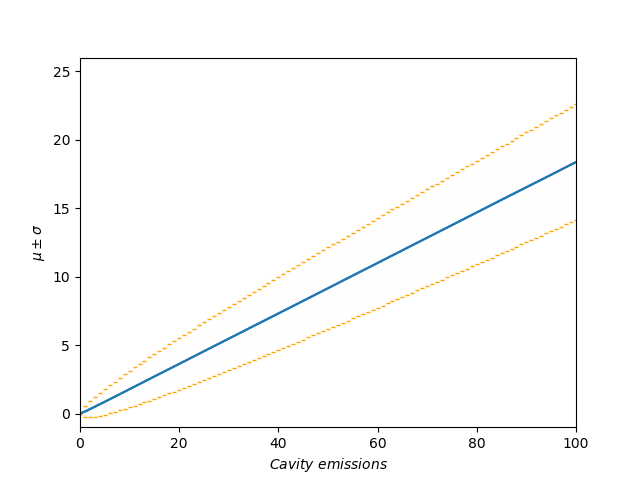
\includegraphics[scale = 0.45]{newsigmaeng.png}
\caption{\small{Average number of spontaneous emissions $\pm \sigma$ with respect to cavity emissions, under parameters $\expval{n} \approx 1$, $\gamma = 1$ , $\kappa = g = 0.1$ and $\mathcal{E} =  \kappa |\langle n \rangle|[1 + 2g^2/\gamma \kappa]$.}}
\label{graph}
\end{figure} 
Having Eq. \eqref{numfo} we are able to stablish a dynamic in the system in which we fix the number of photons. Fixing the photon number to one and leaving $\mathcal{E}$ as a free parameter, we obtain probability distributions of the number of spontaneous emissions $E_i$ for different mean number of spontaneous emissions just as we see in Fig. \ref{probdisult} (a). From these probability distributions we can calculate the variance and graph it against the mean value as we see in Fig. \ref{probdisult} (b), where we obtain a variance almost equal to the mean value, something which is characteristic of Poisson distributions. 
Finally we can graph the mean value of spontaneous emissions against the number of cavity emissions considering standard deviation in order to have a better grasp of the certainty in the estimations, something that is shown in Fig. \ref{graph}.

\section{Correlation between atom and cavity emissions}
So far we have obtained estimations for the number of spontaneous emission for each measured number of cavity emissions. From our results it is obvious how the number of spontaneous emissions will increase with respect to the number of cavity emissions, given that more time will pass and more emissions will occur. One can also see how increasing the cavity linewidth $\kappa$ and keeping the other parameters constant will translate into a decrease of spontaneous emissions with respect to the number of cavity emissions. However, one question remains: is there a direct correlation between these two quantities? If yes, how this varies with respect to the cavity linewidth. From the beginning one could expect that in the case for a big $\kappa$ there would be no correlation at all, since this situation will be equivalent to the situation where there is no cavity. 

In order to have a measure of the correlation of the emissions we introduce the Pearson Correlation Coefficient \cite{benesty2009pearson}
\begin{equation} 
r_{xy} = \frac{\sum\limits_{i=1}^n(x_i - \bar{x})(y_i - \bar{y})}{\sqrt{\sum\limits_{i=1}^n(x_i - \bar{x})^2\sum\limits_{i=1}^n(y_i - \bar{y})^2}}.  \label{correlationc}
\end{equation}
Having an equation that gives us a measure of the correlation, now we want the necessary data in order to obtain information about the correlation between the two types of emissions that we deal with. We can obtain this data by defining a temporal interval from which we make a register of the final number of spontaneous and cavity emissions. Given that what we are doing are essentially stochastic calculations, there will be variations in the final number of emissions for each trajectory. Making a large number of trajectories keeping track of the final number of emissions and pluggin the data in \eqref{correlationc} we are able to calculate the correlation.


\begin{center}
\begin{figure}[t!]
\begin{center}
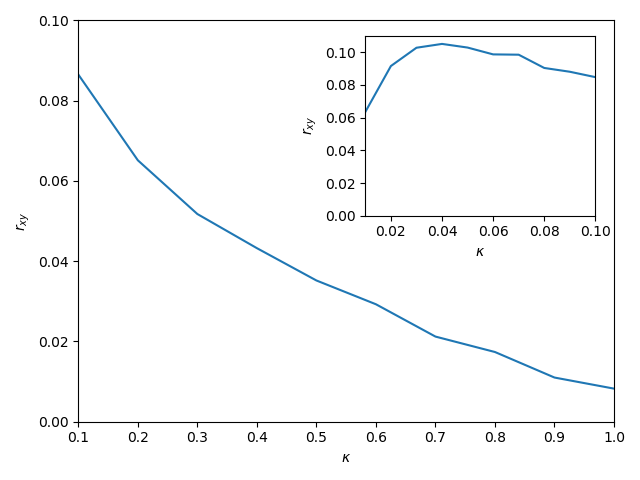
\includegraphics[scale = 0.45]{cor_2.png}
\caption{\small{Calculation of correlation using 500 time intervals, fixing $\expval{n} \approx 1$, $\gamma =$ 1.0, $g = $ 0.1, and with  $\mathcal{E} =  \kappa |\langle n \rangle|[1 + 2g^2/\gamma \kappa]$.}} \label{corrxy}
\end{center}  
\end{figure}
\end{center}

\begin{center}
\begin{figure}[h!]
\begin{center}
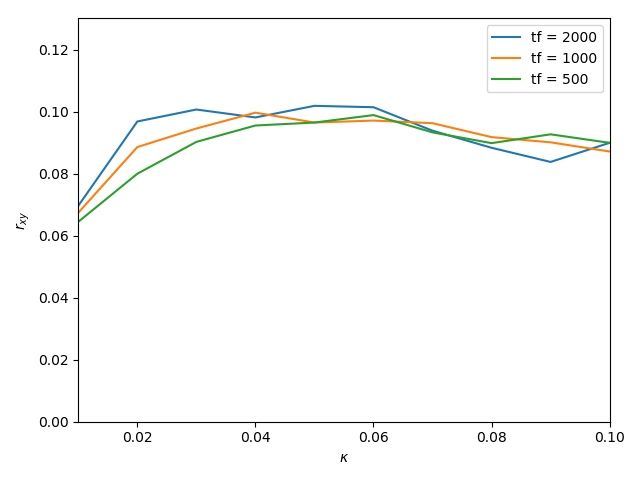
\includegraphics[scale = 0.45]{difftimes12.png}
\caption{\small{Correlation using different temporal intervals, fixing $\expval{n} \approx 1$, $\gamma =$ 1.0, $g =$ 0.1, and with  $\mathcal{E} =  \kappa |\langle n \rangle|[1 + 2g^2/\gamma \kappa]$.}}  \label{errorzz}
\end{center}
\end{figure}
\end{center}
%kncrease or increases
From Fig. \ref{corrxy} we see that, as we expected, the correlation goes to zero as we increase the cavity linewidth. Nonetheless, perhaps a more interesting question is: how high can this correlation be? Trying with values for $\kappa/\gamma$ lower than $0.1$, we notice that the correlation's increase stops and a decrease begins. It is possible that this stop in the increase of the correlation is due to the fact that if we keep decreasing the cavity linewidth it will come a point where the number of emissions will decrease considerably, diminishing the correlation. If this is the case we should expect that as we increase the temporal intervals, %the cavity linewidth at which the correlation starts decreasing should be smaller.
we also see an increment of the correlation.

%In Fig. \ref{errorzz} we can appreciate that, as we increase the total temporal interval, the cavity linewidth at which the correlation starts decreasing is smaller. This supports the idea that the time that takes for the system in stablishing the number photons will affect the minimum value of cavity linewidth at which the correlation starts decreasing.

In Fig. \ref{errorzz} we can appreciate that, as we increase the total temporal interval, there is also a slight increase in the correlation. This supports the idea that the time that takes for the system in stablishing the number photons will affect the value for the correlation, for values of $\kappa/\gamma$ lower than $0.1$.

\section{Conclusions}
In this work we considered a driven Jaynes-Cummings system. We made a program in which, through the use of quantum trajectory theory, we were able to obtain probability distributions that relate the number of spontaneous emissions given certain number of cavity emissions. Through the probability distributions we obtained estimations for the number of spontaneous emissions by measuring cavity emissions, considering the correspondent error. Finally we study the existing correlation where we saw how this correlation decreases as we increase the cavity linewidth. However, if we try with values for  $\kappa/\gamma < 0.1$, there comes a point where the increase stops and we see a decrease. We believe this is related to the fact that if we use enough small values of $\kappa$ there will come a point where the emission of photons will be too low and this will imply a decrease in the correlation. The results in this work provide a tool that could be useful in the manipulation of single photons product of spontaneous emission, and provide insight into the physical behavior of the driven Jaynes-Cummings model.


\section*{Acknowledgment}

Support by UNAM, projects CONACyT and UNAMPAPIIT IG100518.


\bibliographystyle{IEEEtran}
\bibliography{reftesis}
\end{document}
